\chapter{General context}
\label{Chapter1:Intro.Game.Theory}
%\documentclass[10pt]{article}
%\begin{document}

%%%%%%%%%%%%%%%%%%%%%%%%%%%%%%%%%%%%%%%%%%%%%%%%%%%%%%%%%%
%%%%%			Introduction Chapter 1				%%%%%%
%%%%%												%%%%%%
%%%%%												%%%%%%
%%%%%%%%%%%%%%%%%%%%%%%%%%%%%%%%%%%%%%%%%%%%%%%%%%%%%%%%%%

This chapter provides the reader with an introduction to the general context of the work presented in this paper.  Section 2.1 introduces the reader into the basic concepts of cyber security and the kind of cyber security threats that are in scope of this work. Section 2.2 then introduces the reader into the main principles of game theory. Subsequently, section 2.3 introduces the reader to the FlipIt game: this game will be used to model cyber security attacks of a periodic nature, including a delay.  Finally, section 2.4 gives an overview of the related work, and how the research presented in this paper compares to existing results.
%- Remark: to the reader weg
\section{What Is Security?}

Before the digitalization of documents, information was kept on paper and the security of this information was ensured by administrative and physical means. For example, you needed a key to access documents stored in a room full of cabinets where the files were kept. In today's digital era more and more information is kept in a digital format, stored on a computer.  As digitalization progressed, the need for ensuring the security of digital information arose and automated tools were developed to protect files stored on a computer.  

Information security is the generic term for protection of data stored on a computer controlled device such as computers and smartphones, as well as public and private computer networks, including the entire Internet. 
Security is a general term that encompasses several dimensions. More specifically, information security has three fundamental key objectives:

\begin{enumerate}
\item  \textit{Confidentiality}: assuring that the confidentiality of private data is not disclosed or made available to users that do not have proper authorization.
\item \textit{Integrity:} assuring that data cannot be altered by an unauthorized individual.
\item \textit{Availability:} assuring that data is always accessible and that the service is not denied to authorized individuals.
\end{enumerate}



 %The purpose of security is to give certainty that data will not be removed without authorization (Confidentiality) that the data is always accessible (Availability), and that data can not be read or altered by someone who does not have the authorization (Integrity). 
 ~~\\
 These key attributes are also known as the CIA triad. They are the fundamental security objectives for securing data, information and computing services. \\
 \\
Information security can be divided into two main subcategory. One of them is cyber security, also known as computer security. This is the process of applying security tools to ensure confidentiality, integrity, and availability of data. It is an attempt to protect websites, servers, data, applications, operating systems and all assets that need protection in a computer system.  Some of these tools may include detection, identification or removal tools. A detection tool will determine if an infection has taken place and will trace the threat. An identification tool will try to identify the threat to be able to know how to remove it. A removal tool will remove the threat from the system (once it has been identified) so that it cannot spread any further. \\
The other category is network or internet security. This sub category of information security protects data during transmission. While cyber security and network security address different aspects, they partially overlap as well. For example, a virus can be physically dropped on a computer network using a USB stick, but it can also arrive over the internet. Either way internal computer security measurements have to be taken to recover from the virus. In this paper we focus on scenarios where a network has to be defended against attacks to ensure confidentiality, integrity and availability of data. The work presented in this paper therefore belongs to the domain of cyber security.

%hieronder is wel okee


%Cybersecurity attempts to ensure the protection of assets, which includes data, desktops, servers, buildings, and most importantly, humans. The goal of cyber security is to protect data both in transit and at rest. Countermeasures can be put in place in order to increase the security of data. Some of these measures include, but are not limited to, access control, awareness training, audit and accountability, risk assessment, penetration testing, vulnerability management, and security assessment and authorization.'' \todo{tekst overgenomen van wikipedia} \\

\subsubsection{Threats to computer systems}


%In order to keep a system secure and to be able to apply security tools, it is important to mitigate the possible threats. -Remark-Zegt te weinig volgens Matthias 
The possible threats can take many forms, the most common being: spam, malware, spoofing, phishing and  DDoS attacks.  In the context of cyber security, the terms `threat'  and `attack' are often used interchangeably, referring to more or less the same thing. The meaning of these two terms, however, differ slightly from one another. The former refers to anything that can breach security and cause possible harm. It is a possible danger that can exploit a vulnerability. The latter is an assault on computer security that originates from a threat. It is an intelligent act that deliberately tries to breach security through vulnerabilities.  \\

The most noteworthy and biggest group of threats to computer systems is malware. 
This is a piece of malicious software that is designed to penetrate unprotected or vulnerable systems or computers, with the intent to retrieve sensitive information, destroy data, or compromise the confidentiality, integrity or availability of the data or applications of the victim. A security report of 2014 \cite{SurveyKaspersky} reveals that 61\% of the attacks on companies are caused by malware. For this reason this section will examine the categories of malware threats. Different types of malware exist: viruses, worms, flooders, rootkits, bots, spyware, adware and many more. This broad range of different types can be classified into two main categories. The first one based on the propagation method that is used and the second one based on the payload or the variety of actions that the malware performs \cite{stallings2007network}. Propagation methods include viruses, worms and trojans. Payload includes e.g. flooders, rootkits, bots, spyware and adware. This paper focuses on the category of propagation methods and not on the actions that the malware performs. A brief explanation of the three main propagation methods of malware is given below.  

%\begin{figure}[hbtp]
%\caption{2014 survey results by Kaspersky}
%\centering
%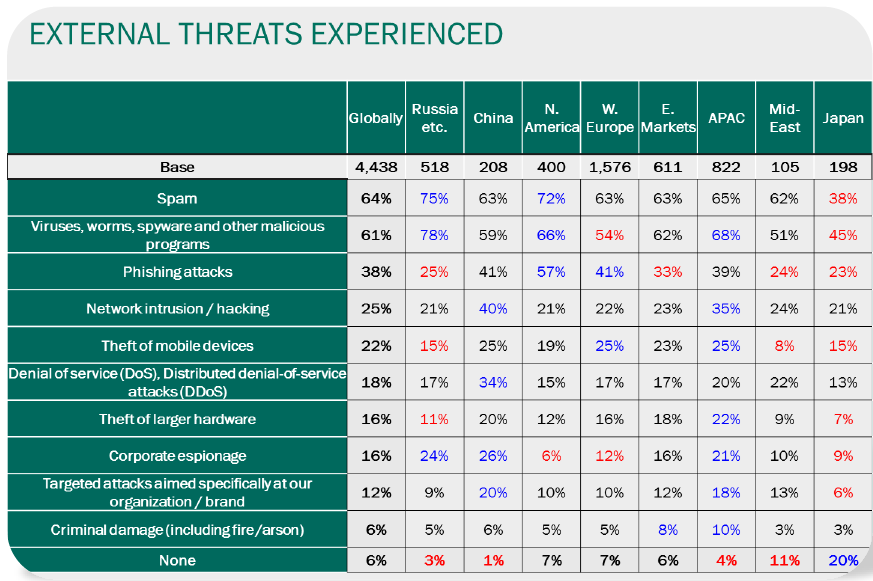
\includegraphics[scale=0.5]{Images/kaspmalware.png}
%\end{figure}

%\begin{table}
%\begin{tabular}{|r|l|}
% \hline
% \textbf{Name}	 & \textbf{Description} \\  \hline 
% Virus & octal \\  \hline 
% Worm & binary \\  \hline 
% Logic bomb
% Trojan Horse
% Backdoor
% Mobile code
% Exploits
% Downloaders
% Auto-rooter
% Kit
%Spammer programs
%Keyloggers
%Flooders
%\end{tabular}
%\caption{Types of Malicious Software, taken over from []}
%\label{table}
%\end{table}
% 
 
\begin{description}
\item \textit{Virus}: This is a malicious piece of code that replicates itself and tries to spread in order  to infect other systems or files. A typical virus will attach itself to a program, or executable content on a computer. The \textit{I love you} virus is an example of a virus where the virus attached itself as an executable to a mail. It propagated by using the mailing systems. When a victim opened an email with the \textit{I love you} virus in the annex, the virus spread itself by sending a mail to everyone in the victim's contact list. 

Using this method, a virus can multiply rapidly, possibly even causing a business network to shut down by the heavy traffic. A virus needs human interaction to spread. In the example above: if no one were to open the mail, the virus would not be able to spread itself and infect other systems.

\item \textit{Worm:} A worm is a virus that can spread without human interaction. It is a computer program that replicates itself in order to spread to other hosts on a network. Copies of the worm can be forwarded via a computer network without an intermediary. The worm will use vulnerabilities of the system to infect other computers.
The \textit{Stuxnetworm} is a very prominent example of a worm. Initially this worm was spread via infected USB sticks and from there on it could spread itself to other hosts on the network through the Internet, without any further human intervention. The purpose of the \textit{Stuxnetworm} was to harm the centrifuges in nuclear reactors; many reactors have been infected.  

\item \textit{Trojan:} This is a malicious program that disguises itself as something normal and useful, so that users won't be suspicious of installing it, but it has a malicious function hidden inside that can circumvent security measures and cause harm.  A notable trojan horse is \textit{Koobface}, that targeted users of Facebook, Skype, Yahoo, Gmail and AOL mail. To spread itself the trojan sent a mail or friend request with a message that directed the recipients to a third party website. This site would then convince the recipient into downloading an update of Adobe Flash Player. Once downloaded and executed, \textit{Koobface }could infect the host.

\end{description}
~~\\
As proposed by Kasperksy \cite{APTKaspersky}, threats caused by the malware described above can be divided into three main categories: known threats (70\%), unknown threats (29\%) and advanced threats (1\%). 

The known threats are the easiest to defend oneself against. Standard malware protection tools like firewalls and virus scanners can keep these kind of malware out of the system. Installing protection against unknown threats is also relatively easy, but this requires tools that go beyond the standard methods, e.g. dynamic whitelisting. The remaining 1\% are the advanced threats, also known as APT. They are the most difficult to deal with.

%-Remark- APTs en niet APT's

\subsubsection{Advanced threats to computer systems}
%\item Backdoors: Also know as trapdoor, is a whole in the system or program that allows access 
%\item Rootkit: A rootkit is designed to be stealthy and hide a set of programs installed on a system from methods of detection.  The programs have administrator or root privileges to that system, which makes it possible to access the functions and services of the operating system, change files, take control over the monitor processes and send and receive network traffic.  A rootkit can make changes to the system to keep itself concealed from detection.

An Advanced Persistent Threat (referred to for the remainder of this work as APT) is a persistent targeted attack that tries to penetrate a network to cause harm while staying unseen for a long period of time. The motive of an APT is mostly cyber espionage, stealing sensitive data, sabotage or other kinds of ideological attacks. APTs are `advanced' because these attacks are well funded and because the attacker (usually) needs a great amount of expertise to successfully penetrate a network. Not all APTs are technically advanced though. The attacker can also try to exploit known vulnerabilities, in the hope that his target has not yet secured itself against them. \\
`Persistent' refers to the fact that the attacker isn't trying to gain immediate results, and the attacker won't stop trying after one failed attempt. The attack can be spread over several years, taking multiple steps.  \\
An APT can be a mix of different types of malware and may use various propagation methods. \\
% like the way a virus, worm or trojan horse propagates. \\
%
%Some examples of the biggest most rare APTs are listed to get an understanding of what APTs are capable of and how long they can stay unseen. [\todo{site kaspersky apt}] 
%
%\subsubsection{Equation}
%Equation is a complex cyberattack platform where the first known sample is from 2002, but it was only discovered 12 years later in 2014. This APT propagates through usb drives, cd or physical media. It will search for exploits and will self-replicate itself to spread the infection. The purpose of this virus is to steal data and cyberespionage. 
%
%\subsubsection{Regin}
%
%\subsubsection{Flame}
%Way of propagation through USB drives, LAN spreading. purpose cyber espionage.
%
%\subsubsection{Black energy}
% purpose cyber espionage and DDoS, data wiping. prop usb lan

 
According to a security survey of Kaspersky \cite{SurveyKaspersky}  the damage of one successful targeted attack against a large company can exceed 2.5 million dollars. As such, companies need a defence mechanism to defend themselves against APTs. As previously stated, simple detection and identification tools are insufficient to protect oneself against APTs, and a removal tool will only work if the threat has been identified. To mitigate these kind of attacks another security countermeasure is needed. \\
%This is where the researchers of RSA come into the picture. \todo{deze paper gaat zien of de game theoretische model kan leiden tot resultaten die kunnen helpen in het verdedigen tegen APTs}
This paper proposes an appropriate game-theoretical modelling of defending a network against APTs and will analyse it in order to draw the necessary strategic conclusions to mitigate these kind of attacks.


\section{A Brief Introduction in Game Theory}
\label{Cha1:briefintro}
%-Remar- based on the work of - Matthias zegt namen erbij zetten
Game theory is a mathematical study to analyse interactions between independent and self-interested agents. To get an understanding of the most important concepts of game theory, a short introduction based on the work of 
\cite{leyton2008essentials} and \cite{Coursera} is given in this section. For a more detailed and complete introduction to game theory, the reader is referred to 
\cite{leyton2008essentials}.  \\
%In section \ref{cha1:FlipItGame} an overview of the FlipIt game is given with the definitions and concepts that will be used throughout the paper. 
%The last section \ref{ch1:extendedWork} will cover the extensions and additions already made on FlipIt. \\
%------------------------------------------------%
%            Intro Game Theory 					 %
%------------------------------------------------%
Game theory is a mathematical way of modelling the interactions between two or more agents where the outcomes depend on what each agent does and and the study of how these interactions should be structured to lead to good outcomes. Game theory therefore has important applications in many areas such as economics, politics, biology, computer science, philosophy and a variety of other disciplines. It gained recognition during the Second World War, when Oskar Morgenstern and John von Neumann both published a book on game theory, titled ``Theory of Games and Economic Behavior'' in 1944 \cite{von1944theory}. This book addressed the mathematical analysis of a series of thinking games. A distinction was made between games in which the strategies and the utility factor of the opponent have no effect on finding the best strategies (e.g. chess) and games wherein this factor does have an influence (e.g. poker). John Nash also played a major role in the history of game theory. He was one of the mathematicians who has formalized game theory. The Nash equilibrium, a common solution concept of a non-cooperative game, was named after him.
~~\\
%Every agent has different levels of happiness for the different outcomes.
%self interested meaning

One of the assumptions underlying game theory is that the players of the game are independent and self-interested. This does not necessarily mean that they want to harm other agents or that they only care about themselves. 
%utility function meaning 
Instead it means that each agent has preferences about which states of the world he likes. These preferences are mapped to natural numbers and are called the utility functions. The numbers are interpreted as a mathematical measure that tells how much an agent likes or dislikes the outcome of the game. Outcomes are the result of a specific combination of a player's strategy. Each combination of a player's strategy is an outcome of the game. \\% The utility function can be ordinal or cardinal. In case of a ordinal utility function only relative rankings are important. The utility function can also be cardinal which is important for games with mixed strategies. \\

%Cooperative and non cooperative games
%-Remark- Stuk herschrijven-- Payoff introduceren -- zin van wikipedia
%Binnen de speltheorie is een 'spel' een (model van) interactie tussen spelers die individueel beslissingen nemen. De spelers ontvangen een beloning (pay-off) die afhangt van hun eigen beslissingen maar ook van die van de anderen. De volgende typen kunnen worden onderscheiden.
%
%Coöperatieve spellen en niet-coöperatieve spellen[bewerken]
%Het verschil tussen deze twee typen spellen is dat bij coöperatieve spellen (cooperative game theory) bindende afspraken tussen de spelers gemaakt kunnen worden terwijl dit niet mogelijk is bij de niet-coöperatieve spellen (non-cooperative game theory).
%The choices of each agent produce an outcome, with respect to the utilities of the agent. A pay-off of an agent is the 
\todo{utility, pay-off, outcomes}
Games can be divided into two types of games: cooperative or non-cooperative. In a non cooperative game, the basic modelling unit is the group of agents. 
Two or more agents want to maximise their utility and their actions can be affected by other agents' utilities. In the individualistic approach the basic modelling is only one agent. This type of game is referred to as \textit{cooperative game theory}. 

%There are two standard representations for games. The first one is the Normal Form. The second one is the Extensive Form.
 

%Nash equilibrium

%John Nash speelde ook een grote rol in de geschiedenis van de speltheorie. Hij is een van de wiskundigen geweest die speltheorie geformaliseerd heeft. Het Nash evenwicht werd naar hem vernoemd. Een Nash evenwicht wordt gezien als een evenwicht tussen beide spelers zodat ze allebei de beste tactiek kiezen en niet meer veranderen als de andere van tactiek veranderen. John Nash breide de theorie over het Nash evenwicht in een paper nog uit met gemengde strategieën. In 1994 kreeg John Nash samen met twee andere wiskundigen gespecialiseerd op het vlak van speltheorie de Nobelprijs voor de economie op basis van hun prestaties in de niet-coöperatieve speltheorie. . Over John Nash is een prachtige film 
\subsubsection{Best Response and Nash Equilibrium}
One of the solution concepts in game theory for non-cooperative games that will be used in this paper is a Nash equilibrium. A Nash Equilibrium is a subset of outcomes that can be interesting to analyse a game. To define this concept we first introduce the concept of best response. The best response, given an action of the other player, is the action that maximizes its pay-off.  We define $Opt_{i}$ as the best response function for player \textit{i}. The best response for player \textit{1} is: $a_{1} = Opt_{1}(a_{2})$, given that $a_{2}$ is an action of player 2. For a Nash Equilibrium each player has a list of actions and each player's action maximizes his or her pay-off given the actions of the other players. Nobody has the incentive to independently or unilaterally change his or her action if an equilibrium profile is played. We have a Nash Equilibrium for the pair $(a_{1}^{*},a_{2}^{*})$ when $a_{1}^{*} = Opt_{1}(a_{2}^{*})$ and $a_{2}^{*} = Opt_{2}(a_{1}^{*})$.\\

%-Remark- Matthias: Beter uitleggen: the best response, given an action of the other player, is the action that maximizes its pay-off. Anders lijk je de definitie  v.e. dominante strategie te geven. (Een actie die ongeacht de actie v.d. tegenstander de beste pay-off geeft) Maak onmiddelijk duidelijk dat het een functie van de acties van de tegenstander betreft. Zo is een dominante actie een actie a waarvoor geldt forall a2 : Opt(a2) = a.
% -Remark- Matthias: Hier moet ‘independently’ of ‘one-sidedly’ of ‘unilateraly’ bij staan, anders beschrijf je een dominante strategie. Het mag voor beide beter zijn om gezamelijk te veranderen, maar niet om unilateraal te wijzigen! Kijk maar naar ’t prisoners dilemma: eenzijdig wisselen is slecht voor iedereen in het T/T Nash equilibrium, maar beide weizigen naar S/S zou voor beiden positief zijn!

An example to explain a Nash equilibrium of a two-player game is the prison dilemma. In this game there are two players who are both rational and both of them have committed a crime. `Rational' means that they want the best for themselves and it is not their purpose to do harm to others. Both are locked in a separate room and they cannot tell in advance to each other what they are going to say. Each of them can betray the other or they can support each other and remain silent. If a player talks, he will either be imprisoned for 3 years or go free, depending on whether the other talks. If the player is silent, he will either be imprisoned for 5 years or one year, depending on whether the other talks.  

%Because betraying a partner offers a greater reward than cooperating with him, all purely rational self-interested prisoners would betray the other, and so the only possible outcome for two purely rational prisoners is for them to betray each other.[1] The interesting part of this result is that pursuing individual reward logically leads both of the prisoners to betray, when they would get a better reward if they both cooperated. 

Figure \ref{Prison} shows the rewards of the possible actions of the two players. The figure shows that it is advantageous for each player to talk (betraying the other). If prisoner 1 talks and the other prisoner remains silent, prisoner 1 will be free. If prisoner 1 remains silent and the other prisoner talks, prisoner 1 gets five years in prison. If the prisoners cooperate and talk, both of them get three years in prison. If they both remain silent they will both get one year in prison. So this means that talking is the dominant strategy. A dominant strategy is a strategy that is better than all other strategies regardless of what the opponent does. The Nash equilibrium of the game is that they both talk even though it would be better if both prisoners cooperated and choose to stay silent. 

\begin{figure}[hbtp]
\centering
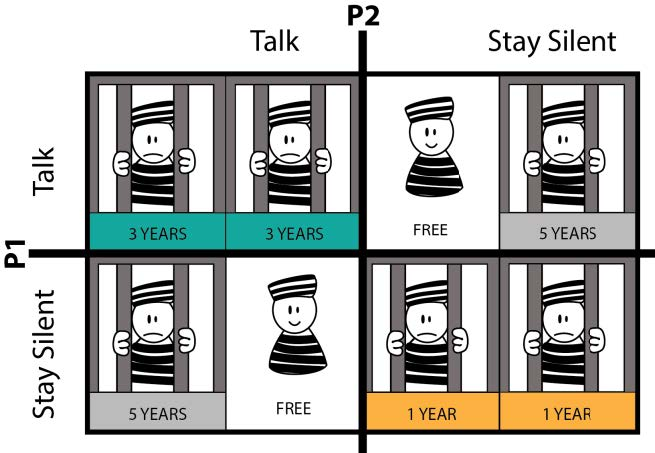
\includegraphics[scale=0.6]{Images/PrisDilemma}
\caption{Prisoners dilemma: An example from the field of Game Theory. It is a game between two perfectly rational prisoners who do not know what the other one will do. Each prisoner can talk (betraying the other) or remain silent. The resulting sentence is shown below each prisoner. }
\label{Prison}
\end{figure}

%In game theory, the Nash equilibrium is a solution concept of a non-cooperative game involving two or more players, in which each player is assumed to know the equilibrium strategies of the other players, and no player has anything to gain by changing only their own strategy.[1] If each player has chosen a strategy and no player can benefit by changing strategies while the other players keep theirs unchanged, then the current set of strategy choices and the corresponding payoffs constitutes a Nash equilibrium. The reality of the Nash equilibrium of a game can be tested using experimental economics method.

%In de speltheorie, een deelgebied van de wiskunde, is een Nash-evenwicht een oplossingsconcept voor een niet-coooperatief spel, waar twee of meer spelers aan meedoen. In een Nash-evenwicht wordt elke speler geacht de evenwichtsstrategieeen van de andere spelers te kennen en heeft geen van de spelers er voordeel bij om zijn of haar strategie eenzijdig te wijzigen. Als elke speler een strategie heeft gekozen en geen enkele speler kan profiteren door zijn strategie te veranderen, terwijl de andere spelers dat ook niet doen, dan vormt de huidige verzameling van strategiekeuzes plus de bijbehorende uitbetalingen een Nash-evenwicht. 

%Een Nash-evenwicht gaat uit van een spel, waarin iedere speler een strategie heeft. Die strategie geeft precies aan wat een speler in de verschillende fases van een spel doet. Een strategie kan zowel een pure strategie als een gemengde strategie zijn. De verzameling van strategieeen van alle spelers die meedoen aan een bepaald spel noemt men een strategieprofiel. In de speltheorie is een Nash-evenwicht een strategieprofiel waarbij het voor geen enkele speler voordelig is daarvan af te wijken, als de andere spelers dat ook niet doen.

%Het Nash-evenwichtsconcept is een begrip dat vooral toepassing vindt in de economie.

%\subsubsection{List of terms}
%The following is a list with the main terms of game theory that will be used throughout the paper.
%\begin{description}
%\item \textit{Players}: Players are referred as the ones who are the decision makers. It can be a person, a company or an animal.  (they are assumed to act rational )
%\item \textit{Actions}: Every player has actions that he or she can do. 
%\item \textit{Strategies}: A strategy is the combination of different actions. A pure strategy consists of only one action.
%\item \textit{Utility}: The utility function or also known as the pay-off is the mapping of the level of happiness of an agent about the state of the world to natural numbers.
%
%\end{description}
%
%A game in game theory consists of multiple agents and every agent has a set of actions that he can play.
\section{The FlipIt Game}
\label{cha1:FlipItGame}
FlipIt is a game introduced by van Dijk et al. To understand how to model a FlipIt game with virus propagation it is important to get familiar with the concepts of the normal FlipIt game and its notations.  Therefore, we first explain the framework of FlipIt and introduce the most important formulas that will be used throughout the paper. \\

FlipIt is a two-players game with a shared single resource that the players want to control as much as possible (figure \ref{fig:FLipItDefault}). The shared resource can be a password, a network or a secret key depending on the setting being modelled. In the remainder of the paper we name the two players the attacker, denoted by the subscript \textit{A} and the defender, denoted by subscript \textit{D}. 

The game begins at $t=0$ and continues indefinitely ($t \rightarrow \infty $). The time in the game is assumed to be continuous. To get control over the resource, the players $i$, with $i \in \{A,D\}$, can flip the resource at any given time. 
%A flip will be regarded as a move from a player \textit{i}. 
Each move implies a certain cost $k_{i}$ and can vary for each player. Both players try to minimize their cost. Adding a cost prevents players from moving too frequently. \\

The unique feature of FlipIt is that every move happens in a stealthy way, meaning that the player does not immediately finds out if the other player (his adversary) has flipped the resource or not. A player only finds out about the state of the game when he moves himself. The goal of the player is to maximize the time that he or she has control over the resource while minimizing the total cost of the moves. A move can also result in a "wasted move", called a flop. It may happen that the resource was already under control of the player. If the player moves when he or she has already control over the resource, he or she would have wasted a move since this does not result in a change of ownership, so the cost is wasted. \\


\begin{figure}[hbtp]
\centering
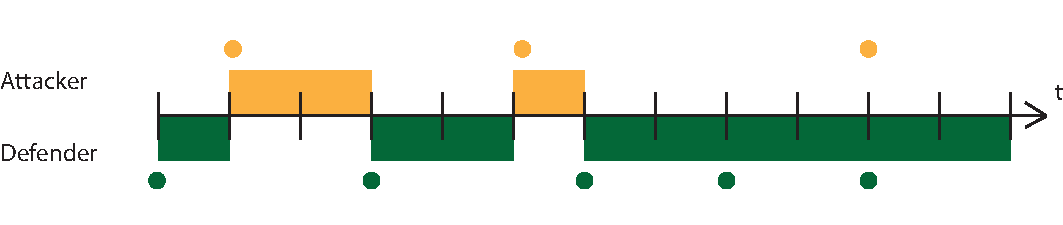
\includegraphics[scale=0.7]{../../doc/template/Images/FlipBasic}
\caption{A representation of a FlipIt game where both players are playing periodically. Every move or flip is indicated by a green (dark grey) or orange (light grey) circle. The attacker is represented in orange and the defender is represented in green. The blue and orange rectangles represent which player is in control of the resource.}
\label{fig:FLipItDefault}
\end{figure}



We denote the state of the resource as a time-dependent variable $C=C_{i}(t)$. 
$C_{D}(t)$ is 1 if the game is under control by the defender and 0 if the game is under control by the attacker. Reversely, $C_{A}(t)$ is 1 if the game is under control by the attacker and 0 if under control by the defender. So, $C_{A}(t)= 1 - C_{D}(t)$.
The game starts with the defender being in control: $C_{D}(0)= 1$. \\



The total gain for player \textit{i} is equal to the total amount of time that player \textit{i} has owned the resource from the beginning of the game up to time \textit{t}:
\begin{equation}\label{first}
G_{i}(t) = \int_0^t \! C_{i}(x) dx.
\end{equation}
The gain of the attacker and the defender always sums up to \textit{t}:
\begin{equation}\label{first}
G_{D}(t) + G_{A}(t) = t
\end{equation}
The average gain rate of player \textit{i} is defined as:
\begin{equation}\label{first}
\gamma_{i}(t) = G_{i}(t)/t.
\end{equation}
And thus for all $t > 0$ :
\begin{equation}\label{first}
\gamma_{D}(t) + \gamma_{A}(t) = 1
\end{equation}
The players receive a benefit equal to the time units they were in possession of the resource minus the cost of making their moves. 
\begin{equation}\label{first}
\beta_{i}(t) = \gamma_{i}(t) - k_{i}\alpha_{i}.
\end{equation}
where  $\beta_{i}(t)$ denote player's \textit{i} average benefit rate, $k_{i}$ denotes the cost for player \textit{i} and $\alpha_{i}$ defines the average move rate by player \textit{i} up to time \textit{t} with $n_{i}(t)$ the amount of moves made by player \textit{i} up to time \textit{t}:
\begin{equation}
\alpha_{i}(t) = \dfrac{n_{i}(t)}{t}
\end{equation}
In a given game, the asymptotic benefit rate (or simply benefit) will be defined as the \textit{lim inf} of the average benefit because time\textit{ t} will increase to infinity and the average benefit may not have limiting values.
\begin{equation}
\beta_{i}(t)  = \lim_{t \to \infty} inf \beta_{i}(t) 
\end{equation}
\\


\subsubsection{Strategies}
Because the players move in a stealthy way, there are different types of feedback a player can get by flipping the resource. These types of feedback can be divided into two groups of strategies. The non-adaptive strategies and the adaptive strategies. These are described in table \ref{table:Strategies}.\\

If there is no feedback for either player, he will play in the same manner against every opponent. The strategy is then called \textit{non-adaptive} because the playing strategy is not dependent on the opponent's movements. An interesting subclass of the non-adaptive strategies are the Renewal strategies where the time intervals between two consecutive moves are generated by a renewal process. The length between two consecutive moves are independent and identically distributed random variables chosen from a density formula \textit{f}. This renewal process means that the strategies are renewed after each move: the interval until the next move only depends on the current move time and not on previous history. \todo{check comment in latex}
%-Remark- Vorige zin is gecopypaste van FlipIt
An example of such renewal strategy is the periodic strategy where the time between two consecutive moves of the players is a fixed interval. An exponential strategy is a renewal strategy in which the interval between two consecutive moves is exponentially distributed. \\

If the players receive feedback, a player can adapt his strategy to the information received about the opponent's moves. This strategy is called \textit{adaptive} strategies. Depending on the amount of information received, two subclasses of adaptive strategies can be identified. The Last Move (LM) strategies represent the class where, whenever a player flips, he will find out the exact moment that the opponent moved the last time. In the second class, called Full History (FH), whenever a player flips he will find out the whole history of the opponent's moves. \\


 \begin{table}
 \centering
 \begin{tabular}{ l | c  }
  \textbf{Categories} & \textbf{Classes of Strategies} \\
  \hline Non-adaptive (NA) & Renewal \\
  & - Periodic \\
  & ~~~ - Exponential \\
  & General non-adaptive \\
  \hline Adaptive (AD) & Last move (LM) \\
  & Full History (FH) \\  
\end{tabular}
 \caption{Hierarchy of Classes of strategies in FlipIt}
 \label{table:Strategies}
 \end{table}

\subsubsection{Results of the FlipIt game}
The study of the different strategies by means of FlipIt framework allows to derive a number of interesting results \cite{FlipIt}:  
\begin{itemize}
\item periodic strategy strongly dominates the other renewal strategies if the opponent has a periodic or non-arithmetic renewal strategy. This means that it is a good choice for the opponent to play periodically against a player with a non-adaptive strategy;
\item periodic games are disadvantageous against players following a Last Move adaptive strategy. The opponent can observe the exact time of the player's next move and play immediately afterwards. If the costs are from the same magnitude, the opponent can keep the control over the resource with little interrupts from the other player; 
\item a player facing an LM opponent and with a cost much lower than the opponent has two options. The first option is to move with a periodic rate that is fast enough he'll force the opponent to drop out. The other option is to play with a randomized strategy, such that the opponent cannot learn any information regarding the next move of the player;
\item the best defence strategy is to play fast, to make the opponent drop out of the game. To be able to move fast, the player has to make sure that the cost of moving is much less than the opponents moves.
%-Remark- Matthias: Hoe is ‘exponential strategy’ randomized? En uitgebreider spreken over de condities: een defender facing an LM attacker and comparable cost…
%\item any amount of feedback about the opponent received during the game, benefits to a player.
\end{itemize}
%-Remark- Matthias: Wat is ‘benefits the player’? Als de speler de feedback negeert benefit die info de speler niet. Ik zou zeggen ‘any amount of feedback about the opponent received during the game allows for better strategies/leads to a better strategy’ ofzo. Let op: Dit is een sterkere/straffere uitspraak, dus denk hier wel goed over na natuurlijk!
 
% In this paper we restrict ourselves to non-adaptive periodic strategies. This choice is motivated by the fact that in a security game a player (defender or attacker) rarely has information about the moves (last move or full history) of his opponent. The results \cite{FlipIt} also indicate that the periodic strategy might be the dominant strategy.  \\

 
\section{Related Work on Extensions to FlipIt}
\label{ch1:extendedWork}

Various possible ways to extend FlipIt have already been proposed. 
Laszka et al. made a lot of additions and extensions to the original game of FlipIt. For instance Laszka et al. extended the basic FlipIt game to multiple resources. The rationale is that for compromising a system in real life, more than just one resource needs to be taken over. For example, gaining access to deeper layers of a system may require breaking several passwords. This model is called FlipThem \cite{FlipThem}. Laszka et al. also use two ways to flip the multiple resources: the AND and the OR control model. In the AND model the attacker only controls the system if he controls all the resources of the system, whereas in the OR model the attacker only needs to compromise one resource to be in control of the entire system. \\

Another addition of Laszka et al. to the game of FlipIt \cite{MitigationCovert} 
is extending the game to also consider non-targeted attacks by non-strategic players. In this game the defender tries to maintain control over the resource that is subjected to both targeted and non-targeted attacks. Non-targeted attacks can include phishing, while targeted attacks may include threats delivered through zero day attack vulnerabilities. \\
One of the last important additions from Laszka et al. \cite{MitigationNonTargeted} is to consider a game with targeted and non-targeted attacks where the moves made by the attacker do not succeed immediately. This approach is similar to what will be done in this paper, but nevertheless has some major differences. Firstly, in Laszka's paper, the moves by the attacker are still covert but the moves made by the defender are known to the attacker. This means that the attacker knows when the defender plays and can change its strategy depending on the moves of the defender. Our motivation for a defender with stealthy moves is that it can not be assumed that every attacker can receive feedback from an APT. Some ATP's are designed only to cause harm on the systems that are infected e.g. the Stuxnetworm that was developed to destroy nuclear reactors. The Stuxnetworm was resident on a isolated network, meaning that there was no way to connect to the internet. Another example is the use of honeypots. Honeypots emulate services or create multiple instances of real operating systems and can pretend to have sensitive information.  Honeypots do not detect all malicious attacks so the attacker can stay unnoticed and can still provide information as feedback. By providing false information through honeypots, the defender can also remain stealthy. The second difference is that even though both the targeted and non-targeted attacks do not succeed immediately, the delay is determined differently. For the targeted attack the time till it succeeds is given by an exponential distributed random variable with a known rate. The non-targeted attacks are modelled as a single attacker and the time until it succeeds is given by a Poisson process. In this paper the delay is given by one parameter, which can be the result of any virus propagation model. The third and last difference is that the paper of Laska has multiple attackers who try to find the best strategy of the defender against both targeted and non-targeted attacks. The conclusion of this paper is that the optimal strategy for the defender is moving periodically. \\ 

FlipIt also has been applied to several cases in computer security. Researchers explored different applications of FlipIt for real-world problems, like password reset policies, VM refresh, cloud auditing and key rotation \cite{ApplyingFlipit}. \\
Other authors used the FlipIt game to apply it to a specific scenario. To be able to use the FlipIt game, modifications were required for the FlipIt model.
One of the scenarios by Pham \cite{compromised} was to find out whether a resource was compromised or not by the attacker. This could be verified by the defender, who has an extra move ``test'' beside the flip move. The basic idea is to test with an extra action if the resource has been compromised or not. This move also involves an extra cost.\\
A three-player game has also been investigated where the FlipIt framework of two players is extended by another player. This player represents an insider that trades value information with the attacker \cite{fengstealthy}.\\


Finally, researchers have also investigated the behaviour of humans playing FlipIt. A. Nochenson and Grossklags \cite{nochenson2013behavioral}  investigated how people really act when given temporal decisions. They found out that the results improve over time but that they are dependent on gender, age, and other individual difference variables. The result also shows that the participants perform generally better when they have more information about the strategy of the opponent, which is a computerized player. Reitter et al. \cite{reitter2013risk} extended the work of A. Nochenson and Grossklags to include various visual presentation modalities for the available feedback during the investigation.\\




% --------------- example of a game -----------------%


%------------------------------------------------%
%            Intro about viruses				 %
%------------------------------------------------%

